
\section*{Motivace a úvod}

Vítame vás u studijního textu k předmětu BI-AG1. Tento text je neoficiální materiál pro tento předmět. Pokud byste narazili na jakoukoli chybu, prosím kontaktujte nás ať ji můžeme opravit.

Jak jistě víte, svět se mění (a to nejen v IT). Díky pokročilým LLM již často není programování "jednoduchých" funkcí už úkolem pro vás, ale pro jazykový model. Proto je ale o to důležitější umět navrhovat a pochopit algoritmy, proč a jak fungují a jak jejich korektnost ověřit jinak, než velkým počtem testovacích dat (ty někdy nemusí stačit, také chybu nemusí vůbec odhalit, nebo ji odhalí až potom, co celý algoritmus dokončíte a zjistíte, že musíte začít znovu). \\

Tento předmět se také věnuje grafům. Je možné, že jste na ně už při studiu narazili, byť možná jen v omezené míře. Ať už v BI-PA2 nebo jako diagram relace v BI-DML. Ale to není zdaleka vše kde se s grafy potkáte. Grafy jsou opravdu všude. Mapa pražského metra? Model počítačové sítě? Hledání cesty v bludišti? Rodokmen? Ano to vše jsou grafy. Tím, že nějaký problém v životě budete reprezentovat grafem a nad ním provádět operace/pouštět algoritmus ho můžete mnohem jednodušeji vyřešit. Například hledání trasy v navigaci je jen hledání nejkratší cesty v grafu. Dají se tím ale řešit i problémy které s grafem zdánlivě nemají ale vůbec nic společného. Například převozníkův problém se dá řešit pomocí reprezentace v grafu a hledáním cesty mezi dvěma vrcholy. \\

Toto se tedy v tomto kurzu naučíte, pojďme ale k věci a konečně si přesně zadefinovat co to takový graf je.

\newpage

\section{1. Přednáška}
\subsection{Základy teorie grafů}

\noindent Jak už jsme zmiňovali, budeme se zde zabývat grafy. Proto si nyní první z nich zavedeme.

\begin{definition}[Neorientovaný graf]
Graf $G$ je uspořádaná dvojice $(V, E)$, kde:
\begin{itemize}
    \item $V$ je neprázdná konečná množina \textbf{vrcholů},
    \item $E$ je množina \textbf{hran}, přičemž každá hrana je dvouprvková podmnožina $V$ (čili neuspořádaná dvojice vrcholů), značíme $\{u, v\}$.
\end{itemize} \medskip
Množinu všech dvouprvkových podmnožin množiny $V$ (tedy všech možných hran) značíme $\binom{V}{2}$. \medskip
\end{definition}

Všimněte si, že díky vlastnosti množin, nemůže být více hran mezi dvěma vrcholy a nezáleží na pořadí vrcholů v množině hrany. 

\begin{center}
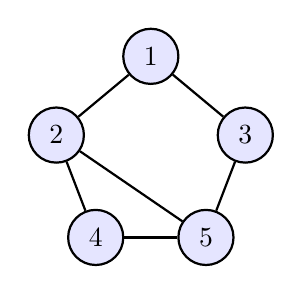
\begin{tikzpicture}[
  vnode/.style={circle, draw, minimum size=7mm, inner sep=0pt, fill=blue!10},
  thick
]
  \node[vnode] (1) at (0, 1.5) {1};
  \node[vnode] (2) at (-1.2, 0.5) {2};
  \node[vnode] (3) at (1.2, 0.5) {3};
  \node[vnode] (4) at (-0.7, -0.8) {4};
  \node[vnode] (5) at (0.7, -0.8) {5};
  
  \draw (1) -- (2);
  \draw (1) -- (3);
  \draw (2) -- (4);
  \draw (3) -- (5);
  \draw (4) -- (5);
  \draw (2) -- (5);
\end{tikzpicture}
\par\medskip
\textit{Obrázek 1.1: Příklad neorientovaného grafu s 5 vrcholy a 6 hranami.}

\end{center}


\begin{remark}
\begin{enumerate}
    \item Množinu vrcholů grafů zavádíme jakožto neprázdnou. Důvodem je aby jsme u většiny důkazů nemuseli explicitně ošetřovat prázdný graf. Poté u datových struktur toto omezení pomineme.
    \item Množina hran je vždy dvouprvková podmnožina vrcholů. Díky tomu, že je množinou, tak nám vylučuje případ \{$v$, $v$\}, kde $v \in V$ nějakého grafu G. Tedy neorientovaný graf nemůže obsahovat smyčky, tedy hranu na jednom vrcholu.
\end{enumerate}
\end{remark}

\bigskip

\begin{definition}[Značení a incidence]
Nechť $e = \{u, v\}$ je hrana v grafu $G$. Pak řekneme, že:
\begin{itemize}
    \item vrcholy $u$ a $v$ jsou \textbf{koncové vrcholy} hrany $e$,
    \item $u$ je \textbf{sousedem} $v$ v $G$ (a naopak),
    \item $u$ i $v$ jsou \textbf{incidentní} s hranou $e$.
\end{itemize}
Počet vrcholů grafu budeme obvykle značit $n = |V(G)|$ a počet hran $m = |E(G)|$.
\end{definition}

\begin{center}
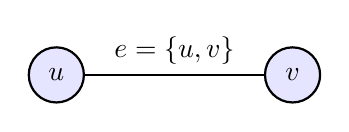
\begin{tikzpicture}[
  vnode/.style={circle, draw, minimum size=7mm, inner sep=0pt, fill=blue!10},
  thick
]
  \node[vnode] (u) at (0, 0) {$u$};
  \node[vnode] (v) at (3, 0) {$v$};
  \draw (u) -- node[above] {$e = \{u, v\}$} (v);
\end{tikzpicture}
\par\medskip
\textit{Obrázek 1.2: Vizualizace incidence vrcholu a sousedství přes hranu $e$.}
\end{center}

\bigskip

\begin{definition}[Sled a cesta]
\textbf{Sled} délky $k$ v grafu $G$ je sekvence $v_0, e_1, v_1, e_2, \dots, e_k, v_k$ taková, že $e_i = \{v_{i-1}, v_i\}$ a $e_i \in E(G)$ pro všechna $i = 1, \dots, k$. \\
\textbf{Cesta} v grafu $G$ je sled, ve kterém se neopakují vrcholy (a tedy ani hrany). \\
Má-li cesta $P$ v grafu $G$ koncové vrcholy $s = v_0$ a $t = v_k$, mluvíme o \textbf{cestě z $s$ do $t$} (nebo o \textbf{$s$-$t$-cestě}). Připouštíme i $s = t$ (cesta nulové délky). \\
\textbf{Délka} $s$-$t$-cesty je počet hran v této cestě. \\
\textbf{Vzdálenost} $s$ a $t$, značná $d(s, t)$, je délka nejkratší $s$-$t$-cesty v grafu $G$.
\end{definition}

\begin{center}
    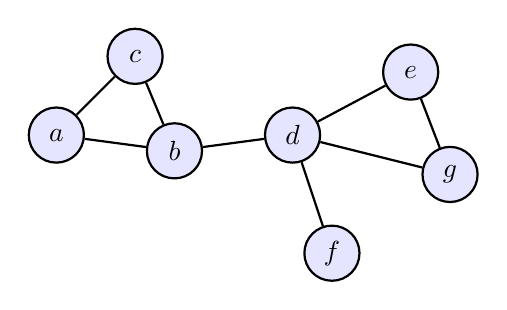
\begin{tikzpicture}[
  vnode/.style={circle, draw, minimum size=7mm, inner sep=0pt, fill=blue!10},
  thick
]
  \node[vnode] (a) at (0, 1) {$a$};
  \node[vnode] (c) at (1, 2) {$c$};
  \node[vnode] (b) at (1.5, 0.8) {$b$};
  \node[vnode] (d) at (3, 1) {$d$};
  \node[vnode] (e) at (4.5, 1.8) {$e$};
  \node[vnode] (g) at (5, 0.5) {$g$};
  \node[vnode] (f) at (3.5, -0.5) {$f$};
  
  \draw (a) -- (b);
  \draw (a) -- (c);
  \draw (c) -- (b);
  \draw (b) -- (d);
  \draw (d) -- (e);
  \draw (e) -- (g);
  \draw (g) -- (d);
  \draw (d) -- (f);
\end{tikzpicture}
\par\medskip
\textit{Obrázek 1.3: Sekvence $a, b, d, e, g, d, f$ je sled, ale ne cesta (opakuje se vrchol $d$). Sekvence $a, b, d, f$ je cesta.}
\end{center}

\newpage

\subsection{Algoritmus BFS (Breadth-First Search)}

\noindent Nyní si představíme velmi důležitý algoritmus BFS neboli Breath-First search. Ten slouží pro nalezení nejkratší cesty mezi vrcholy. S jeho znalostí, pokud převedeme náš problém na graf, tak zvládneme najít nejkratší řešení.

\noindent \textbf{Vstup}: Neorientovaný graf $G = (V, E)$ a počáteční vrchol $s \in V$. \newline
\noindent \textbf{Výstup}:
\begin{itemize}[itemsep=-0.2em, topsep=0.1em]
    \item Pole vzdáleností $D$ od vrcholu $s$ takové, že:
    \begin{itemize}[itemsep=-0.15em, label=$\bullet$]
        \item $D[v] = k$, kde $k$ je délka nejkratší $s$-$v$-cesty v $G$,
        \item $D[v] = \text{undef}$, pokud neexistuje žádná $s$-$v$-cesta v $G$.
    \end{itemize}
    \item Pole předchůdců $P$ takové, že:
    \begin{itemize}[itemsep=-0.15em, label=$\bullet$]
        \item $P[v] = w$, kde $w$ je předchůdce $v$ na nějaké nejkratší $s$-$v$-cestě v $G$,
        \item $P[v] = \text{undef}$, pokud neexistuje žádná $s$-$v$-cesta v $G$.
    \end{itemize}
\end{itemize}

Tedy algoritmus má najít délky nejkratších cest mezi počátčním vrcholem $s$ a všemi ostatními. Pokud se ptáte, jak získat samotnou nejkratší cestu (tedy posloupnost vrcholů a hran), tak tu lze jednoduše získat díky poli předchůdců $P$, stačí se podívat na předchůdce posledního vrcholu a následně jeho předchůdce a toto opakovat dokud se nedostaneme do samotného vrcholu $s$. Hledaná cesta je pak posloupnost těchto předchůdců.


\noindent \textbf{Jak funguje BFS}: Začneme v počátečním vrcholu s. Poté vezmeme všechny jeho ještě nenalezené sousedy a umístíme je do fronty. Na závěr vrchol s uzavřeme a jeho práce končí. Následně opakujeme:
\begin{enumerate}
    \item Vezmeme první prvek ve frontě, nazvěmě ho $v$.
    \item Přidáme hodnotu do pole vzdáleností a pole předchůdců pro vrchol $v$
    \item Přidáme do fronty všechny zatím nenalezené sousedy vrcholu $v$ a nastavíme je jako otevřené
    \item Označíme $v$ jako uzavřený
\end{enumerate}
Jakmile již neni možné vzít další prvek z fronty (fronta je prázdná) algoritmus končí. Výstupem jsou naplněná pole vzdáleností a předchůdců. Pro ilustraci se můžete podívat do slidů z přednášky, nebo na některé z mnoha videí dostupných na internetu. Pseudokód pak vypadá takto: \bigskip

\funkce{BFS}{graf $G$, vrchol $s$}
\begin{pseudocode}
\item Pro každý vrchol $v \in V(G)$:
\item \tab $\text{stav}[v] := \text{nenalezený}$
\item \tab $D[v] := \text{undef}$
\item \tab $P[v] := \text{undef}$
\item $Q := \text{fronta obsahující jediný vrchol } s$
\item $\text{stav}[s] := \text{otevřený}$
\item $D[s] := 0$
\item $P[s] := \bot$
\item Dokud je fronta $Q$ neprázdná:
\item \tab Vyjmi z $Q$ první vrchol, nechť to je $v$
\item \tab Pro všechny sousedy $w$ vrcholu $v$:
\item \tab \tab Pokud $\text{stav}[w] = \text{nenalezený}$:
\item \tab \tab \tab $\text{stav}[w] := \text{otevřený}$
\item \tab \tab \tab $D[w] := D[v] + 1$
\item \tab \tab \tab $P[w] := v$
\item \tab \tab \tab Přidej $w$ na konec fronty $Q$
\item \tab $\text{stav}[v] := \text{uzavřený}$
\item Vrať $(D, P)$
\end{pseudocode} \bigskip

\noindent Nyní co jsme algoritmus zavedli, tak je potřeba ho analyzovat. Dokazuje se většinou několik vlastností. Zejména konečnost, že algoritmus někdy doběhne a správnost tedy že výsledek co dostaneme je správný. Nyní začneme konečností. \bigskip

\begin{theorem}[O konečnosti algoritmu BFS]
Algoritmus $BFS(G, s)$ se vždy zastaví.
\end{theorem}

\begin{proof}
Každý vrchol je přidán do fronty $Q$ nejvýše jednou, neboť před svým vložením je jeho stav změněn na \textit{otevřený} a nemůže již vícekrát splnit podmínku, že je \textit{nenalezený}. V každé iteraci hlavního cyklu je právě jeden vrchol odebrán z fronty. Protože množina vrcholů $V(G)$ je konečná, algoritmus se zastaví nejvýše po $|V(G)|$ iteracích hlavního cyklu.
\end{proof} \bigskip

\begin{definition}[BFS fáze a BFS hladiny]
    \leavevmode\\
    Hladina $H_0 = \{s\}$. Fáze $F_0$ trvá od odebrání $s$ z fronty $Q$, otevření a vložení všech jeho sousedů do $Q$ až do uzavření $s$. \\
    Hladina $H_i$ (pro $i > 0$) je množina všech vrcholů otevřených a vložených do $Q$ ve fázi $F_{i-1}$. \\
    Fáze $F_i$ trvá od konce fáze $F_{i-1}$ až po uzavření všech vrcholů z $H_i$. To zahrnuje vyjmutí všech vrcholů z $H_i$ z fronty $Q$, otevření jejich dosud nenalezených sousedů a vložení těchto sousedů do $Q$. \\
    Nechť $h$ je číslo poslední fáze algoritmu BFS.
\end{definition} \bigskip

\begin{center}
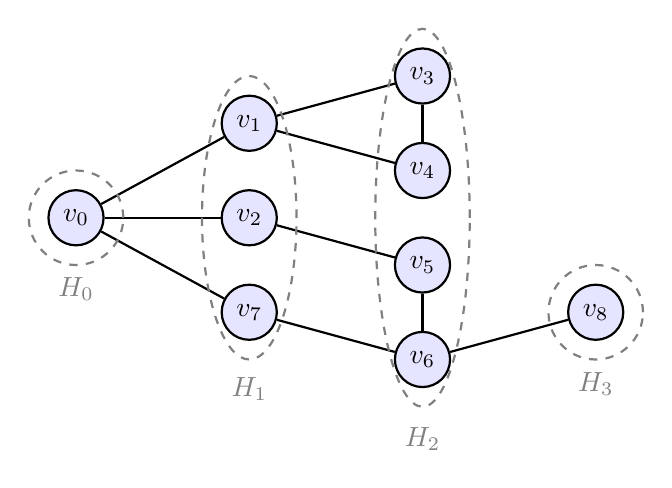
\begin{tikzpicture}[
  vnode/.style={circle, draw, minimum size=7mm, inner sep=0pt, fill=blue!10},
  thick
]
  % Nodes
  \node[vnode] (v0) at (0, 0) {$v_0$};
  
  \node[vnode] (v1) at (2.2, 1.2) {$v_1$};
  \node[vnode] (v2) at (2.2, 0) {$v_2$};
  \node[vnode] (v7) at (2.2, -1.2) {$v_7$};
  
  \node[vnode] (v3) at (4.4, 1.8) {$v_3$};
  \node[vnode] (v4) at (4.4, 0.6) {$v_4$};
  \node[vnode] (v5) at (4.4, -0.6) {$v_5$};
  \node[vnode] (v6) at (4.4, -1.8) {$v_6$};
  
  \node[vnode] (v8) at (6.6, -1.2) {$v_8$};
  
  % Edges
  \draw (v0) -- (v1);
  \draw (v0) -- (v2);
  \draw (v0) -- (v7);
  
  \draw (v1) -- (v3);
  \draw (v1) -- (v4);
  \draw (v2) -- (v5);
  \draw (v7) -- (v6);
  
  \draw (v6) -- (v8);
  
  \draw (v3) -- (v4);
  \draw (v5) -- (v6);
  
  % Elipsy pro hladiny
  \draw[gray, dashed] (0, 0) circle [x radius=0.6, y radius=0.6] node[below=18pt] {$H_0$};
  \draw[gray, dashed] (2.2, 0) ellipse [x radius=0.6, y radius=1.8] node[below=54pt] {$H_1$};
  \draw[gray, dashed] (4.4, 0) ellipse [x radius=0.6, y radius=2.4] node[below=72pt] {$H_2$};
  \draw[gray, dashed] (6.6, -1.2) circle [x radius=0.6, y radius=0.6] node[below=18pt] {$H_3$};
\end{tikzpicture}
\par\medskip
\textit{Obrázek 2.1: Rozklad grafu na hladiny $H_0, H_1, H_2, H_3$ podle vzdálenosti od $v_0$.}
\end{center}

\noindent Nyní si dokážeme korektnost algoritmu. Vždy u korektnosti dokazujeme vše co nám algoritmus slibuje. Zde u BFS jsou to 3 věci, že správně uzavře vrcholy, že správně naplní pole vzdáleností a pole předchůdců. \\

\noindent \textbf{Zde se lišíme od přednášky! V přednášce jsou ty důkazy velmi odmávané, a kdyby byli na zkoušce (jako že tam pravděpodobně nebudou), tak by nemuseli být uznané. Pokud chcete pochopit princip doporučujeme přednášku, zde jsou stejné ale víc formálně popsané}


\begin{theorem}[O správnosti algoritmu BFS]
Po skončení algoritmu $BFS(G, s)$ platí následující vlastnosti pro každý vrchol $v \in V(G)$:
\begin{itemize}
    \item \textbf{Vlastnost 1}: Vrcholy jsou ve stavu \textit{uzavřený} právě tehdy, když do nich ze startu $s$ vede cesta. Ostatní vrcholy zůstanou \textit{nenalezené}.
    \item \textbf{Vlastnost 2}: Pro všechny uzavřené vrcholy $v$ platí $D[v] = d(s, v)$ (délka nejkratší cesty ze startu $s$ do $v$).
    \item \textbf{Vlastnost 3}: Pro všechny uzavřené vrcholy $v \neq s$ platí $P[v] = w$, kde $w$ je předchůdce $v$ na nějaké nejkratší cestě ze startu $s$ do $v$.
\end{itemize}
\end{theorem} \bigskip

\subsubsection{Důkazy správnosti BFS}

\begin{proof}[Důkaz Vlastnosti 1]
Připomínáme, že prvním otevřeným a následně uzavřeným vrcholem je startovní vrchol $s$. Algoritmus otevírá všechny dosud nenalezené sousedy právě zpracovávaného vrcholu. Zmiňme ještě, že dosažitelný vrchol říkáme vrcholu, do kterého existuje cesta z vrcholu $s$ (tedy samotný $s$ toto také splňuje).

Jedná se o ekvivalenci, musíme proto ukázat platnost dvou implikací.

\begin{itemize}
    \item Vrchol $v$ je dosažitelný z $s \implies$ vrchol $v$ bude uzavřen. \\

    \textbf{Základní krok}: Pro cestu délky $0$ platí $v=s$.
    Startovní vrchol $s$ algoritmus otevře na začátku, takže tvrzení platí.

    \textbf{Indukční krok}: Předpokládejme, že každý vrchol, ke kterému
    vede ze $s$ cesta délky $k$, bude otevřen. Uvažujme nyní vrchol $v$,
    ke kterému vede ze $s$ cesta délky $k+1$. Označme $u$ předposlední
    vrchol této cesty. Potom ke $u$ vede ze $s$ cesta délky $k$ a mezi
    $u$ a $v$ existuje hrana.

    Podle indukčního předpokladu bude vrchol $u$ otevřen. Při jeho
    zpracování algoritmus BFS prochází všechny jeho sousedy, tedy i
    vrchol $v$. Pokud $v$ ještě nebyl nalezen, BFS jej otevře. Pokud
    již nalezen byl, byl otevřen dříve. V obou případech tedy bude
    $v$ během algoritmu otevřen.

    \item Vrchol $v$ je uzavřený $\implies$ vrchol $v$ je dosažitelný z $s$ \\
    Tvrzení dokážeme indukcí podle pořadí ve kterém BFS vrcholy otevírá.
    
    \textbf{Základní krok}: Prvním otevřeným vrcholem je vrchol s. Vrchol s je dosažitelný z s cestou délky 0.

    \textbf{Indukční krok}: Předpokládejme, že vrchol u byl otevřen dříve než vrchol v a že u je dosažitelný z s. Vrchol v je otevřen při zpracování vrcholu u, takže mezi u a v existuje hrana {u,v}. Nyní můžeme spojit cestu ze s do u s hranou {u,v}, čímž dostaneme cestu ze s do v. Tedy vrchol v je dosažitelný z s.
\end{itemize}
\end{proof}

\bigskip

\noindent Myšlenka důkazu. Zvolíme fázi $F_i$. Z konstrukce BFS víme, že každý vrchol $v \in H_i$ má vzdálenost od $s$ nejvýše $i$, protože existuje cesta z $s$ do $v$ právě přes $i$ hladin. Zbývá ukázat, že nemůže existovat kratší cesta. Kdyby existovala cesta z $s$ do $v$ kratší než $i$, musela by při průchodu z $H_0$ do $H_i$ přeskočit alespoň jednu hladinu. To ale není možné, protože každé dva sousední vrcholy leží buď ve stejné hladině, nebo v hladinách s rozdílem nejvýše 1.

\begin{proof}[Důkaz Vlastnosti 2]
Důkaz provedeme indukcí dle fáze. \\
\textbf{Základní krok}: Tvrzení triviálně platí pro fázi $F_0$, kde $D[s] = 0 = d(s, s)$. \\
\textbf{Indukční krok}: Uvažujme indukční krok pro fázi $F_i$ kde $i > 0$. Pokud $v \in H_i$, pak podle konstrukce $D[v] = i$ a z $s$ do $v$ existuje cesta o $i$ hranách. Tedy skutečná vzdálenost $d(s, v) \le i$. \\
Nyní ukážeme sporem, že nemůže existovat žádná $s$-$v$-cesta kratší než $i$. Předpokládejme, že existuje cesta $P$ z $s$ do $v$ o délce $j < i$. Protože $j < i$, musí podle holubníkového principu na cestě $P$ existovat dva sousední vrcholy $w$ a $w'$ a dvě nesousední hladiny $H_k$ a $H_\ell$ (tj. $|k - \ell| > 1$) takové, že $w \in H_k$ a $w' \in H_\ell$. \\
To je ovšem spor s tím, že sousední vrcholy na cestě mustí ležet v sousedních hladinách (rozdíl indexů hladin sousedních vrcholů může být nejvýše 1, protože když se zpracovává hladina $H_k$, všichni její dosud nenalezení sousedé se zařadí do $H_{k+1}$, a ostatní sousedé již leží v $H_k$ nebo $H_{k-1}$). \\
Tento spor dokazuje, že žádná kratší cesta neexistuje, a tedy $d(s, v) = i = D[v]$.
\end{proof}

Na závěr této části bychom ještě rádi doporučili vyřešit si miniprogtest na BFS, nejenže díky tomu BFS lépe pochopíte, ale také vám usnadní řešení progtestu velkého.

\subsection{Speciální třídy grafů a vlastnosti}

Nyní si zavedeme pár speciálních grafů o kterých se často budeme bavit. Důležité je jejich značení. Úplný graf je $K_n$, Úplný bipartnitní graf je $K_{n,m}$, Kružnice je $C_n$ a Cesta je $P_n$. Kde n značí počet vrcholů.

\begin{definition}[Úplný graf]
Nechť $n \ge 1$. \textbf{Úplný graf} na $n$ vrcholech, značný $K_n$, je graf $(V, \binom{V}{2})$, kde $|V| = n$. V úplném grafu jsou každé dva různé vrcholy spojené hranou. Někdy se úplné grafy také nazývají klika.
\end{definition}

\begin{figure}[H]
\centering
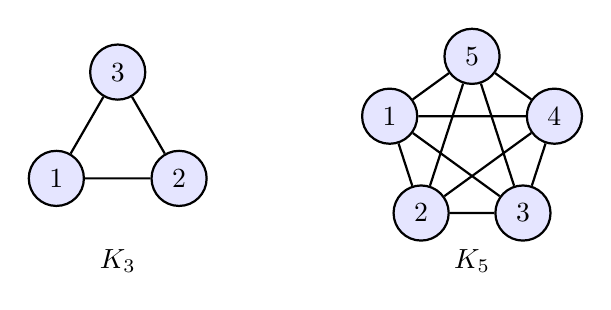
\begin{tikzpicture}[
  vnode/.style={circle, draw, minimum size=7mm, inner sep=0pt, fill=blue!10},
  thick
]
  \begin{scope}[shift={(0,0)}]
    \foreach \i in {1,2,3} {
      \node[vnode] (u\i) at ({90 + \i*360/3}:0.9) {\i};
    }
    \draw (u1) -- (u2) -- (u3) -- (u1);
    \node at (0, -1.5) {$K_3$};
  \end{scope}
  
  \begin{scope}[shift={(4.5,0)}]
    \foreach \i in {1,2,3,4,5} {
      \node[vnode] (w\i) at ({90 + \i*360/5}:1.1) {\i};
    }
    \draw (w1) -- (w2) -- (w3) -- (w4) -- (w5) -- (w1);
    \draw (w1) -- (w3) -- (w5) -- (w2) -- (w4) -- (w1);
    \node at (0, -1.5) {$K_5$};
  \end{scope}
\end{tikzpicture}
\caption{Úplné grafy $K_3$ (3 vrcholy, 3 hrany) a $K_5$ (5 vrcholů, 10 hran).}
\end{figure}

\begin{observation}
 Úplný graf o $n$ vrcholech je $n-1$ regulární. 
\end{observation}

\bigskip

\begin{definition}[Úplný bipartitní graf]
Nechť $n_1 \ge 1$ a $n_2 \ge 1$. \textbf{Úplný bipartitní graf} $K_{n_1,n_2}$ tvořený dvěma partitami o velikostech $n_1$ a $n_2$ je graf $(A \cup B, E)$, kde $A \cap B = \emptyset$, $|A| = n_1$, $|B| = n_2$ a množina hran je:
$$E = \{ \{a, b\} \mid a \in A, b \in B \}$$
Platí, že $|E| = n_1 \cdot n_2$.
\end{definition}

\begin{center}
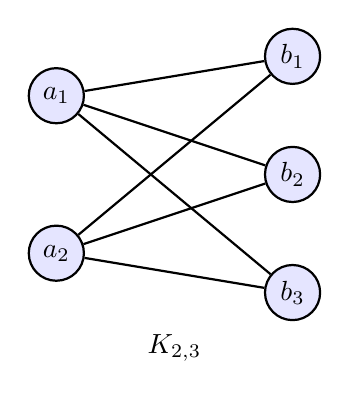
\begin{tikzpicture}[
  vnode/.style={circle, draw, minimum size=7mm, inner sep=0pt, fill=blue!10},
  thick
]
  \node[vnode] (a1) at (0, 1) {$a_1$};
  \node[vnode] (a2) at (0, -1) {$a_2$};
  
  \node[vnode] (b1) at (3, 1.5) {$b_1$};
  \node[vnode] (b2) at (3, 0) {$b_2$};
  \node[vnode] (b3) at (3, -1.5) {$b_3$};
  
  \foreach \i in {1,2} {
    \foreach \j in {1,2,3} {
      \draw (a\i) -- (b\j);
    }
  }
  \node at (1.5, -2.2) {$K_{2,3}$};
\end{tikzpicture}
\par\medskip
\textit{Obrázek 3.2: Úplný bipartitní graf $K_{2,3}$ s partitami velikosti 2 a 3.}
\end{center} 
\bigskip

\begin{definition}[Cesta]
\textbf{Cesta} o $n$ vrcholech (označovaná $P_n$ pro $n \ge 1$) je graf s množinou vrcholů 
$V = \{1, \dots, n\}$ a množinou hran $E = \{ \{i, i+1\} \mid i \in \{1, \dots, n-1\} \}$.
\end{definition}

\begin{figure}[H]
\centering
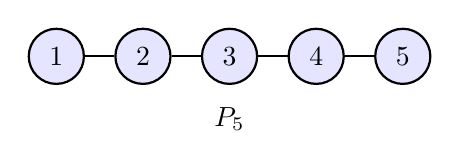
\begin{tikzpicture}[
  vnode/.style={circle, draw, minimum size=7mm, inner sep=0pt, fill=blue!10},
  thick
]
  \foreach \i in {1,2,3,4,5} {
    \node[vnode] (v\i) at ({(\i-1)*1.1}, 0) {\i};
  }
  \draw (v1) -- (v2) -- (v3) -- (v4) -- (v5);
  
  \node at (2.2, -0.8) {$P_5$};
\end{tikzpicture}
\caption{Cesta $P_5$ s pěti vrcholy.}
\end{figure}
\bigskip

\begin{definition}[Kružnice]
\textbf{Kružnice} o $n$ vrcholech (označovaná $C_n$ pro $n \ge 3$) je graf s množinou vrcholů
$V = \{1, \dots, n\}$ a množinou hran $E = \{ \{i, i+1\} \mid i \in \{1, \dots, n-1\} \} \cup \{ \{n,1\} \}.$
\end{definition}

\begin{figure}[H]
\centering
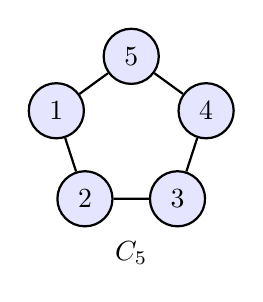
\begin{tikzpicture}[
  vnode/.style={circle, draw, minimum size=7mm, inner sep=0pt, fill=blue!10},
  thick
]
  \foreach \i in {1,2,3,4,5} {
    \node[vnode] (c\i) at ({90 + \i*360/5}:1.0) {\i};
  }
  \draw (c1) -- (c2) -- (c3) -- (c4) -- (c5) -- (c1);
  
  \node at (0, -1.5) {$C_5$};
\end{tikzpicture}
\caption{Kružnice $C_5$ s pěti vrcholy.}
\end{figure}
\bigskip

\begin{definition}[Doplněk grafu]
\textbf{Doplněk} $\bar{G}$ grafu $G = (V, E)$ je graf $(V, \binom{V}{2} \setminus E)$. Obsahuje tedy stejné vrcholy, ale jeho hrany jsou právě ty dvojice vrcholů, které v $G$ netvoří hranu.
\end{definition}

\begin{center}
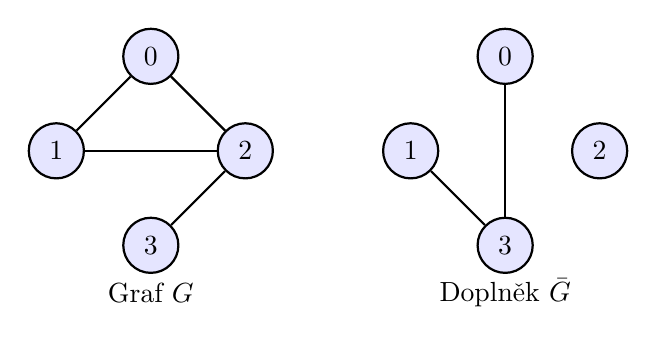
\begin{tikzpicture}[
  vnode/.style={circle, draw, minimum size=7mm, inner sep=0pt, fill=blue!10},
  thick
]
  \begin{scope}[shift={(0,0)}]
    \node[vnode] (0) at (0, 1.2) {0};
    \node[vnode] (1) at (-1.2, 0) {1};
    \node[vnode] (2) at (1.2, 0) {2};
    \node[vnode] (3) at (0, -1.2) {3};
    
    \draw (0) -- (1);
    \draw (0) -- (2);
    \draw (1) -- (2);
    \draw (2) -- (3);
    \node at (0, -1.8) {Graf $G$};
  \end{scope}
  
  \begin{scope}[shift={(4.5,0)}]
    \node[vnode] (0') at (0, 1.2) {0};
    \node[vnode] (1') at (-1.2, 0) {1};
    \node[vnode] (2') at (1.2, 0) {2};
    \node[vnode] (3') at (0, -1.2) {3};
    
    \draw (0') -- (3');
    \draw (1') -- (3');
    \node at (0, -1.8) {Doplněk $\bar{G}$};
  \end{scope}
\end{tikzpicture}
\par\medskip
\textit{Obrázek 3.4: Příklad grafu $G$ a jeho doplňku $\bar{G}$ na čtyřprvkové množině vrcholů.}
\end{center}
\bigskip

\begin{definition}[Okolí a stupně]
Nechť $G = (V, E)$ je graf a $v \in V$ jeho vrchol.
\begin{itemize}
    \item Stupněm vrcholu $v$ v grafu $G$ nazveme počet hran incidentních s ním. Značeno: $\deg_G(v)$.
    \item Symbolem $N_G(v)$ označíme \textbf{otevřené okolí} vrcholu $v$, tj. množinu všech sousedů $v$. Platí $\deg_G(v) = |N_G(v)|$.
    \item Symbolem $N_G[v] = N_G(v) \cup \{v\}$ označíme \textbf{uzavřené okolí} vrcholu $v$.
\end{itemize}
\end{definition}

\begin{figure}[H]
\centering
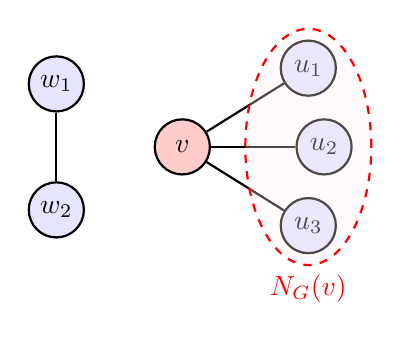
\begin{tikzpicture}[
  vnode/.style={circle, draw, minimum size=7mm, inner sep=0pt, fill=blue!10},
  thick
]
  \node[vnode, fill=red!20] (v) at (0, 0) {$v$};
  
  \node[vnode] (u1) at (1.6, 1) {$u_1$};
  \node[vnode] (u2) at (1.8, 0) {$u_2$};
  \node[vnode] (u3) at (1.6, -1) {$u_3$};
  
  \node[vnode] (w1) at (-1.6, 0.8) {$w_1$};
  \node[vnode] (w2) at (-1.6, -0.8) {$w_2$};
  
  \draw (v) -- (u1);
  \draw (v) -- (u2);
  \draw (v) -- (u3);
  \draw (w1) -- (w2);
  
  \draw[red, dashed, thick, fill=red!5, fill opacity=0.3] (1.6, 0) ellipse [x radius=0.8, y radius=1.5];
  \node[red] at (1.6, -1.8) {$N_G(v)$};
\end{tikzpicture}
\caption{Okolí $N_G(v)$ vrcholu $v$. Vrcholy $w_1$ and $w_2$ nepatří do okolí $v$.}
\end{figure}
\bigskip

\begin{definition}[Regulární graf]
\textbf{Regulární graf} stupně $r$ (neboli $r$-regulární graf) je graf, v němž má každý vrchol stupeň právě $r$.
\end{definition}

\begin{center}
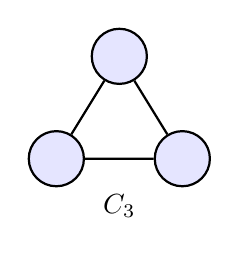
\begin{tikzpicture}[
  vnode/.style={circle, draw, minimum size=7mm, inner sep=0pt, fill=blue!10},
  thick
]
  \node[vnode] (r1) at (0, 0.9) {};
  \node[vnode] (r2) at (-0.8, -0.4) {};
  \node[vnode] (r3) at (0.8, -0.4) {};
  
  \draw (r1) -- (r2) -- (r3) -- (r1);
  
  \node at (0, -1.0) {$C_3$};
\end{tikzpicture}

\par\medskip
\textit{Obrázek 3.6: Příklad 2-regulárního grafu $C_3$.}
\end{center}
\begin{figure}[H]
\centering
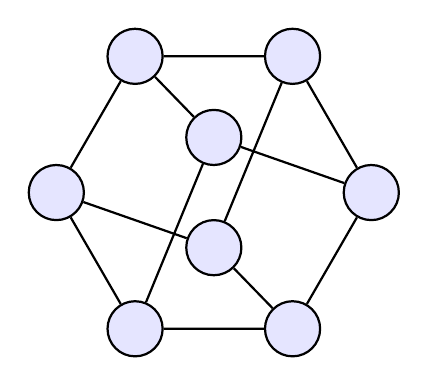
\begin{tikzpicture}[
  vnode/.style={circle, draw, minimum size=7mm, inner sep=0pt, fill=blue!10},
  thick
]
  % C6 cycle vertices (hexagon)
  \node[vnode] (v1) at (2, 0) {};
  \node[vnode] (v2) at (1, 1.73) {};
  \node[vnode] (v3) at (-1, 1.73) {};
  \node[vnode] (v4) at (-2, 0) {};
  \node[vnode] (v5) at (-1, -1.73) {};
  \node[vnode] (v6) at (1, -1.73) {};
  
  % Two internal vertices
  \node[vnode] (c1) at (0, 0.7) {};
  \node[vnode] (c2) at (0, -0.7) {};
  
  % Cycle edges (C6)
  \draw (v1) -- (v2) -- (v3) -- (v4) -- (v5) -- (v6) -- (v1);
  
  % Internal vertex c1 connects to v1, v3, v5
  \draw (c1) -- (v1);
  \draw (c1) -- (v3);
  \draw (c1) -- (v5);
  
  % Internal vertex c2 connects to v2, v4, v6
  \draw (c2) -- (v2);
  \draw (c2) -- (v4);
  \draw (c2) -- (v6);
\end{tikzpicture}
\caption{Příklad 3-regulárního grafu na 8 vrcholech ($C_6$ se dvěma vnitřními vrcholy).}
\end{figure}


\begin{definition}[Izolovaný vrchol]
\textbf{Izolovaný vrchol} je vrchol stupně $0$, tedy vrchol, který nemá žádné sousedy.
\end{definition}



\subsection{Věta o principu sudosti}

Princip sudosti nám říká, že každý graf musí mít dohromady sudý počet stupňů. Proč je to pravda? Každá hrana má dva vrcholy a každý z těchto vrcholů si započítá 1 stupeň. Tedy za každou hranu máme 2 stupně. \newline

\begin{theorem}[O principu sudosti / Handshaking lemma]
Pro každý graf $G = (V, E)$ platí:
$$\sum_{v \in V} \deg_G(v) = 2|E|$$
\end{theorem}

\begin{proof}
Při sečtení stupňů všech vrcholů započítáme každý konec každé hrany právě jednou. Jelikož každá hrana má přesně dva konce, započítáme každou hranu přesně dvakrát.
\par
Formálně to můžeme vyjádřit následujícím řetězcem rovností:
$$\sum_{v \in V} \deg_G(v) = \sum_{v \in V} |N_G(v)| = \sum_{v \in V} |\{u \in V \mid \{u, v\} \in E\}|$$
Tedy součet stupňů všech vrcholů je roven počtu jeho sousedů (přímo definice). \\

To vyjádříme dvěma sumami:

$$\sum_{v \in V} \sum_{\substack{e \in E \\ v \in e}} 1$$

Vnější suma je přes všechny vrcholy $v \in V(G)$ a vnitřní suma sčítá přes všechny hrany současného vrcholu $v$.

Prohozením pořadí sumace (přesčítáním přes všechny hrany a jejich konce, tedy vždy 2 vrcholy):
$$\sum_{e \in E} \sum_{v \in e} 1 = \sum_{e \in E} 2 = 2|E|$$

Dostáváme požadovaný počet.
  \end{proof}

\bigskip

\begin{corollary}
Z věty o principu sudosti plynou tyto důležité vlastnosti:
\begin{enumerate}
    \item V každém grafu je počet vrcholů lichého stupně sudý.
    \item Každý regulární graf lichého stupně musí mít sudý počet vrcholů.
\end{enumerate}
\end{corollary}

Princip sudosti nám dává nutnou podmínku která se, jak už to jistě znáte, skvěle hodí pro vyvracení existence grafů. Pokud byste například dostali za úkol sestrojit graf tak, aby obsahoval vrcholy se zadanými stupni, pokud součet stupňů bude lichý hned víte, že to nelze (nemusíte sčítat samotné stupně, stačí se jen podívat na počet vrcholů s lichým stupněm a pokud jich nebude sudě tak víte, že součet stupňů musí být taky lichý). Také se tato věta velmi hodí u důkazů sporem, kde často můžete nalézt spor právě s touto větou.

\bigskip

\noindent Teď si zavedeme podgrafy. Podgraf je podmnožina původního grafu, ale pouze tak že je stále grafem. Důležité: prázdný graf neni grafem a celý graf je podgrafem sama sebe. \\
Více omezení jsme u indukovaného podgrafu, který po vybrání podmnožiny vrcholů musí zahrnout všechny hrany co mezi libovolnou dvojicí z nich vedli.

\medskip

\begin{definition}[Podgraf a indukovaný podgraf]
\leavevmode\\
Graf $H$ je \textbf{podgrafem} grafu $G$ (píšeme $H \subseteq G$), pokud $V(H) \subseteq V(G)$ a $E(H) \subseteq E(G)$. \\
Graf $H$ je \textbf{indukovaným podgrafem} grafu $G$, pokud $V(H) \subseteq V(G)$ a množina hran $E(H)$ obsahuje právě ty hrany z $G$, které mají oba koncové vrcholy ve $V(H)$, tedy:
$$E(H) = E(G) \cap \binom{V(H)}{2}$$
Indukovaný podgraf na množině vrcholů $V' \subseteq V$ značíme $G[V']$. \\
Graf $G - V'$ značí podgraf indukovaný množinou $V \setminus V'$. Pro jednoprvkovou množinu píšeme zkráceně $G - v$. \\
Podgraf úplného bipartitního grafu se nazývá \textbf{bipartitní graf}.
\end{definition}

\begin{figure}[H]
\centering
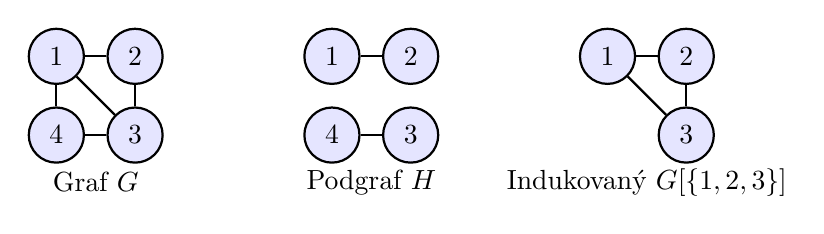
\begin{tikzpicture}[
  vnode/.style={circle, draw, minimum size=7mm, inner sep=0pt, fill=blue!10},
  thick
]
  % G
  \begin{scope}[shift={(0,0)}]
    \node[vnode] (1) at (0, 1) {1};
    \node[vnode] (2) at (1, 1) {2};
    \node[vnode] (3) at (1, 0) {3};
    \node[vnode] (4) at (0, 0) {4};
    \draw (1) -- (2);
    \draw (2) -- (3);
    \draw (3) -- (4);
    \draw (4) -- (1);
    \draw (1) -- (3);
    \node at (0.5, -0.6) {Graf $G$};
  \end{scope}
  
  % Podgraf H
  \begin{scope}[shift={(3.5,0)}]
    \node[vnode] (1') at (0, 1) {1};
    \node[vnode] (2') at (1, 1) {2};
    \node[vnode] (3') at (1, 0) {3};
    \node[vnode] (4') at (0, 0) {4};
    \draw (1') -- (2');
    \draw (3') -- (4');
    \node at (0.5, -0.6) {Podgraf $H$};
  \end{scope}
  
  % Indukovaný podgraf G[V'] pro V' = {1, 2, 3}
  \begin{scope}[shift={(7,0)}]
    \node[vnode] (1'') at (0, 1) {1};
    \node[vnode] (2'') at (1, 1) {2};
    \node[vnode] (3'') at (1, 0) {3};
    \draw (1'') -- (2'');
    \draw (2'') -- (3'');
    \draw (1'') -- (3'');
    \node at (0.5, -0.6) {Indukovaný $G[\{1,2,3\}]$};
  \end{scope}
\end{tikzpicture}
\caption{Příklad grafu $G$, jeho podgrafu $H$ (chybí některé hrany) a indukovaného podgrafu na množině vrcholů $\{1, 2, 3\}$ (obsahuje všechny dostupné vnitřní hrany).}
\end{figure}

\bigskip

\begin{definition}[Klika]
\textbf{Klika} v grafu $G$ je podmnožina vrcholů $C \subseteq V(G)$, v níž jsou každé dva vrcholy spojené hranou (čili indukovaný podgraf $G[C]$ je úplný graf).
\end{definition}

\begin{center}
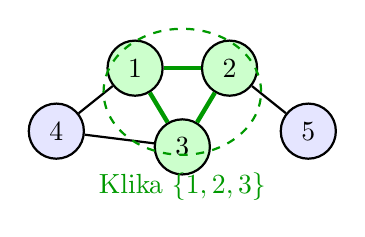
\begin{tikzpicture}[
  vnode/.style={circle, draw, minimum size=7mm, inner sep=0pt, fill=blue!10},
  thick
]
  \node[vnode, fill=green!20] (1) at (0, 1) {1};
  \node[vnode, fill=green!20] (2) at (1.2, 1) {2};
  \node[vnode, fill=green!20] (3) at (0.6, 0) {3};
  \node[vnode] (4) at (-1, 0.2) {4};
  \node[vnode] (5) at (2.2, 0.2) {5};
  
  \draw[green!60!black, ultra thick] (1) -- (2);
  \draw[green!60!black, ultra thick] (2) -- (3);
  \draw[green!60!black, ultra thick] (3) -- (1);
  
  \draw (1) -- (4);
  \draw (3) -- (4);
  \draw (2) -- (5);
  
  \draw[green!60!black, dashed] (0.6, 0.7) circle [x radius=1.0, y radius=0.8];
  \node[green!60!black] at (0.6, -0.5) {Klika $\{1,2,3\}$};
\end{tikzpicture}
\par\medskip
\textit{Obrázek 5.2: Graf obsahující kliku velikosti 3 (zvýrazněná zeleně).}
\end{center}

\bigskip

\noindent Na závěr si zavedeme druhý typ grafu a to orientovaný graf. V orientovaném grafu řešíme směr, vrcholu z říkáme předchůdce a vrcholu po říkáme následník. A navíc nám oproti neorientovanému dovoluje smyčky. Tedy hranu na jednom vrcholu. Tyto grafy stále splňují vše co jsme si zavedli.

\begin{definition}[Orientovaný graf]
\textbf{Orientovaný graf} $G$ is uspořádaná dvojice $(V, E)$, kde:
\begin{itemize}
    \item $V$ is neprázdná konečná množina \textbf{vrcholů},
    \item $E$ is množina \textbf{orientovaných hran}. Orientovaná hrana $e = (u, v)$ is uspořádaná dvojice vrcholů $u, v \in V$ (zobrazujeme jako šipku z $u$ do $v$).
\end{itemize}
Říkáme, že $u$ je \textbf{předchůdce} $v$ a $v$ je \textbf{následník} $u$. \\
Orientovaná hrana tvaru $(u, u)$ se nazývá \textbf{smyčka}.
\end{definition}

\begin{center}
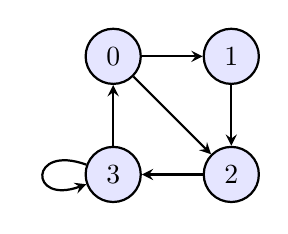
\begin{tikzpicture}[
  vnode/.style={circle, draw, minimum size=7mm, inner sep=0pt, fill=blue!10},
  thick,
  >=stealth
]
  \node[vnode] (0) at (0, 1.2) {0};
  \node[vnode] (1) at (1.5, 1.2) {1};
  \node[vnode] (2) at (1.5, -0.3) {2};
  \node[vnode] (3) at (0, -0.3) {3};
  
  \draw[->] (0) -- (1);
  \draw[->] (1) -- (2);
  \draw[->] (2) -- (3);
  \draw[->] (3) -- (0);
  \draw[->] (0) -- (2);
  \draw[->] (3) to [out=160, in=200, looseness=8] (3);
\end{tikzpicture}
\par\medskip
\textit{Obrázek 5.3: Příklad orientovaného grafu se smyčkou na vrcholu 3.}
\end{center} \bigskip

\noindent BFS lze poměrně lehce modifikovat, tak že přijímá i orientované grafy. Stačí nahradit sousedy za následníky, jelikož neuvažujeme sousedy ze kterých jde šipka k nám. \bigskip

\funkce{\textcolor{red}{BFS-Orientovaný}}{\textcolor{red}{orientovaný} graf $G$, vrchol $s$}
\begin{pseudocode}
\item Pro každý vrchol $v \in V(G)$:
\item \tab $\text{stav}[v] := \text{nenalezený}$
\item \tab $D[v] := \text{undef}$
\item \tab $P[v] := \text{undef}$
\item $Q := \text{fronta obsahující jediný vrchol } s$
\item $\text{stav}[s] := \text{otevřený}$
\item $D[s] := 0$
\item $P[s] := \bot$
\item Dokud je fronta $Q$ neprázdná:
\item \tab Vyjmi z $Q$ první vrchol, nechť to je $v$
\item \tab Pro všechny \textcolor{red}{\textbf{následníky}} $w$ vrcholu $v$:
\item \tab \tab Pokud $\text{stav}[w] = \text{nenalezený}$:
\item \tab \tab \tab $\text{stav}[w] := \text{otevřený}$
\item \tab \tab \tab $D[w] := D[v] + 1$
\item \tab \tab \tab $P[w] := v$
\item \tab \tab \tab Přidej $w$ na konec fronty $Q$
\item \tab $\text{stav}[v] := \text{uzavřený}$
\item Vrať $(D, P)$
\end{pseudocode}

\newpage

\subsection{Modifikace BFS - První zápočtovka}
